\documentclass[tikz]{standalone}
\usetikzlibrary{positioning, arrows.meta}
\begin{document}
    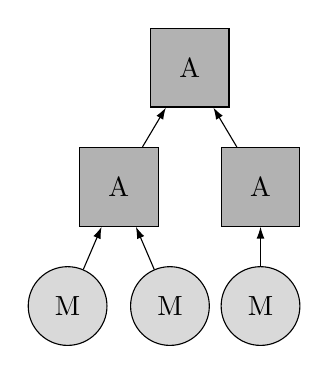
\begin{tikzpicture}[
        A/.style = {draw, black, fill=black!30, minimum height=1cm, minimum width=1cm, inner sep=2pt},
        M/.style = {draw, black, fill=black!15, circle, minimum size=1cm, inner sep=2pt},
        arrow/.style = {-{Latex[length=1.5mm, width=1.0mm]},align=flush center}
    ]
        
        \node[A] (A) {A};

        \node[A, below=0.5cm of A, xshift=-0.9cm] (Al) {A};
        \node[M, below=0.5cm of Al, xshift=-0.65cm] (Ml) {M};
        \node[M, below=0.5cm of Al, xshift=0.65cm] (Mr) {M};


        \node[A, below=0.5cm of A, xshift=0.9cm] (Ar) {A};
        \node[M, below=0.5cm of Ar] (M) {M};

        \draw[arrow] (M) -> (Ar);
        \draw[arrow] (Ml) -> (Al);
        \draw[arrow] (Mr) -> (Al);
        \draw[arrow] (Al) -> (A);
        \draw[arrow] (Ar) -> (A);


    \end{tikzpicture}
\end{document}